\PassOptionsToPackage{unicode,pdfusetitle}{hyperref}
\PassOptionsToPackage{hyphens}{url}
\PassOptionsToPackage{dvipsnames,svgnames*,x11names*}{xcolor}

\documentclass[10pt,ignorenonframetext]{beamer}

\usepackage{lmodern}
\usepackage{amssymb,amsmath,mathtools,amsthm}
\usepackage[T1]{fontenc}
\usepackage[utf8]{inputenc}
\usepackage{textcomp} % provide euro and other symbols

\usepackage{pgfpages}

\usepackage{multirow}
\usepackage{csvsimple}
\usepackage{siunitx}

% prevent slide breaks in the middle of a paragraph
\widowpenalties 1 10000
\raggedbottom


% Use upquote if available, for straight quotes in verbatim environments
\usepackage{upquote}
\usepackage[]{microtype}
\UseMicrotypeSet[protrusion]{basicmath} % disable protrusion for tt fonts

\usepackage{xcolor}
\usepackage{xurl} % add URL line breaks if available
\usepackage{bookmark}
\usepackage{hyperref}
\hypersetup{
  colorlinks = true,
  linkcolor  = Maroon,
  filecolor  = Maroon,
  citecolor  = Blue,
  urlcolor   = Blue
}

% tikz and pgfplots stuff
\usepackage{tikz}
\usetikzlibrary{arrows,shapes,positioning,intersections}
\usepackage{pgfplots}
\usepgfplotslibrary{external,colormaps}
\pgfplotsset{width=7cm,compat=1.11}
%\tikzexternalize

\newif\ifbibliography
\setlength{\emergencystretch}{3em} % prevent overfull lines
\setcounter{secnumdepth}{-\maxdimen} % remove section numbering

%\usepackage{subfig}
\usepackage{subcaption}
\usepackage{algorithm,algpseudocode}
\usepackage{booktabs}


% biblatex
\usepackage[citestyle=authoryear]{biblatex}
\addbibresource{references.bib}

\AtBeginPart{\frame{\partpage}}
\AtBeginSection{\ifbibliography\else\frame{\sectionpage}\fi}
\AtBeginSubsection{\frame{\subsectionpage}}

\usetheme{boxes}
\usecolortheme{beaver}
\usefonttheme{professionalfonts}
\usefonttheme{structurebold}
\setbeamertemplate{footline}[frame number]
\setbeamertemplate{caption}[numbered]
\setbeamertemplate{caption label separator}{: }
\setbeamercolor{caption name}{fg=normal text.fg}
\setbeamertemplate{itemize item}{\(\bullet\)}
\setbeamertemplate{itemize subitem}{\(\circ\)}
\setbeamertemplate{itemize subsubitem}{\textendash}
\setbeamerfont{frametitle}{size=\large}
\setbeamerfont{framesubtitle}{size=\small}
% \setbeamertemplate{headline}{\vskip4ex}
\beamertemplatenavigationsymbolsempty

% operators
\DeclareMathOperator*{\argmax}{arg\,max}
\DeclareMathOperator*{\argmin}{arg\,min}
\DeclareMathOperator{\sign}{sign}
\DeclareMathOperator{\E}{E}
\DeclareMathOperator{\var}{Var}

% macros
\newcommand{\pkg}[1]{\textsf{#1}}
\renewcommand{\vec}[1]{\bm{#1}}
\newcommand{\mat}[1]{\bm{#1}}
\newcommand{\du}{\mathrm{d}}



% title block
\title{The Hessian Screening Rule and Adaptive Paths for the Lasso}
\subtitle{Statistics Seminar at the Department of Mathematical Statistics,
  Chalmers/Gothenburg University}
\author{Johan Larsson}
\institute{Department of Statistics, Lund University}
\date{\today}
\titlegraphic{\includegraphics{figures/logo.pdf}}

\begin{document}

\frame[noframenumbering,plain]{\titlepage}

\begin{frame}{Overview}
  \tableofcontents[hideallsubsections]
\end{frame}

\section{Preliminaries}

\begin{frame}{The Lasso}
  The lasso~\parencite{tibshirani1996} is a type of penalized regression,
  represented by the following
  convex optimization problem:
  \[
    \operatorname*{minimize}_{\beta \in \mathbb{R}^p}
    \left\{
      f(\beta) + \lambda \lVert \beta \rVert_1.
    \right\}
  \]
  where \(f(\beta)\) is smooth and convex.

  \begin{columns}[c]
    \begin{column}{0.45\linewidth}
      \(f(\beta) = \frac 1 2 \lVert y - X\beta\rVert_2^2\)
      leads to the ordinary lasso \medskip

      \(\lambda\) is a hyper-parameter that controls the level of
      \alert{penalization}.
      \medskip

      \(\hat\beta(\lambda)\) is the solution to this problem for a given
      \(\lambda.\)

    \end{column}
    \begin{column}{0.45\linewidth}
      \begin{figure}
        \centering
        \pgfplotsset{width=6cm,height=6cm}
        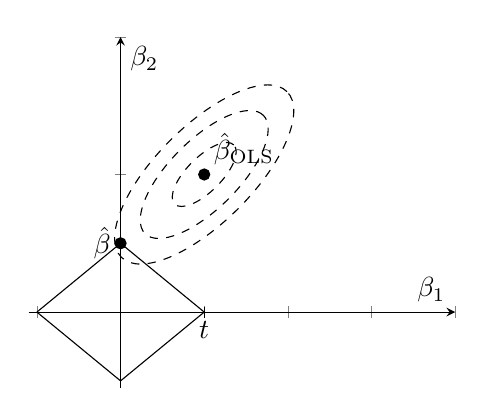
\begin{tikzpicture}
\begin{axis}[
    xlabel = \(\beta_1\),
    ylabel = \(\beta_2\),
    ymin = -1.1,
    ymax = 4,
    xmin = -1.1,
    xmax = 4,
    axis lines = center,
    yticklabels={,,},
    xticklabels={,,}
]
\draw[dashed, rotate around={45:(1,2)}] (1,2) ellipse (0.5 and 0.25);
\draw[dashed, rotate around={45:(1,2)}] (1,2) ellipse (1 and 0.5);
\draw[dashed, rotate around={45:(1,2)}] (1,2) ellipse (1.4 and 0.7);

\addplot[]
    coordinates {
    	(-1,0)
    	(0,1)
    	(1,0)
    	(0,-1)
    	(-1,0)
    };
    
\addplot [only marks, mark=*] coordinates {(1,2)};
\node [above right,black] at (1,2) {\(\hat\beta_\text{OLS}\)};

\addplot [only marks, mark=*] coordinates { (0,1) };
\node [left] at (0,1) {$\hat\beta$};

\addplot [only marks, mark = |] coordinates { (1, 0) };
\node [below] at (1,0) {\(t\)};
\end{axis}
\end{tikzpicture}
        \caption{Level-curves and constraints for two-variable OLS}
      \end{figure}
    \end{column}
  \end{columns}
\end{frame}

\begin{frame}{The Lasso Path}
  % \(\lambda \in [\lambda_\text{max}, 0)\) traces a set of
  % solutions.
  varying \(\lambda \in [0, \infty)\) traces the set of all solutions for the
  lasso---the (exact) lasso path. \medskip

  In practice, we start at the all-sparse solution,
  \(\hat\beta(\lambda_\text{max}) = 0\) and finish at some fraction of
  \(\lambda_\text{max}\) where the model is almost saturated. \medskip

  \pause

  This set of solutions is piece-wise linear with breaks occurring whenever the
  active set, the support set of the non-zero regression coefficients
  corresponding to \(\hat\beta(\lambda)\), changes. \medskip

  The size of the active set cannot exceed \(n\), the number of observations.
\end{frame}

\begin{frame}
  \begin{figure}
    \includegraphics{figures/lasso-path}
    \caption{The lasso path for an example of the standard lasso}
  \end{figure}
\end{frame}

\begin{frame}{Picking \(\lambda\)}

  \begin{block}{The Problem}
    We (typically) don't know the optimal value for
    \(\lambda\). To tackle this, we use cross-validation to tune for
    \(\lambda\).
  \end{block}

  \pause

  \medskip

  \begin{block}{Grid Search}
    In our problem domain (\(p \gg n\)), the standard procedure is to create a
    grid of \(\lambda\)s and fit the lasso iteratively.
  \end{block}

  \medskip

  \pause

  This can, however, get computationally demanding when the number of
  predictors, \(p\) is large. In our target domain, it may not even be possible
  to fit the data set into memory.

\end{frame}

\subsection{Screening Rules}

\begin{frame}{Predictor Screening Rules}
  \begin{block}{Motivation}
    Many of the solution vectors, \(\hat\beta\),
    along the regularization path will be \alert{sparse}, which means some
    predictors (columns) in \(X\) will be \alert{inactive}, especially
    if \(p \gg n\).
  \end{block}
  \pause
  \begin{block}{Basic Idea}
    Say that we are at step \(k\) on the lasso path and are about to solve for
    step \(k + 1\). \medskip

    Intuitively, the information at step \(k\) should give us some information
    about which predictors are going to be non-zero at step \(k + 1\). \medskip

    The idea is to use this information to \alert{discard} a subset of the
    predictors and fit the model to a smaller set of predictors---the screened
    set.
  \end{block}
\end{frame}

\begin{frame}{Types of Screening Rules}
  \begin{block}{Safe Rules}
    Provides a certificate that discarded predictors will be inactive at the
    optimum.
  \end{block}
  \pause
  \begin{block}{Heuristic (Un-Safe) Rules}
    May result in \alert{violations}: discarding predictors that actually will
    be active. Requires post-optimization checks of optimality conditions.
    \medskip

    Checking the optimality conditions requires recomputing the full gradient,
    which is costly.
  \end{block}
\end{frame}

\begin{frame}{Optimality Conditions}
  \(\beta\) is a solution to the lasso problem if it satisfies the stationarity
  criterion
  \[
    \boldsymbol{0} \in \nabla f(\beta) + \lambda \partial
  \]
  where \(\partial\) is the subdifferential of \(\lVert \beta \rVert_1\),
  defined as
  \[
    \partial_j \in
    \begin{cases}
      \{\sign(\beta_j)\} & \text{if } \beta_j \neq 0, \\
      [-1,1]             & \text{otherwise.}
    \end{cases}
  \]
  \pause
  This means that
  \[
    |\nabla f(\beta)_j| < \lambda \implies \hat\beta_j = 0.
  \]
  Of course, we don't know \(\nabla f(\beta)\) prior to solving the problem.

  % TODO: insert subdifferential plot
\end{frame}

\begin{frame}{The Gradient Perspective of the Path}
  \begin{figure}
    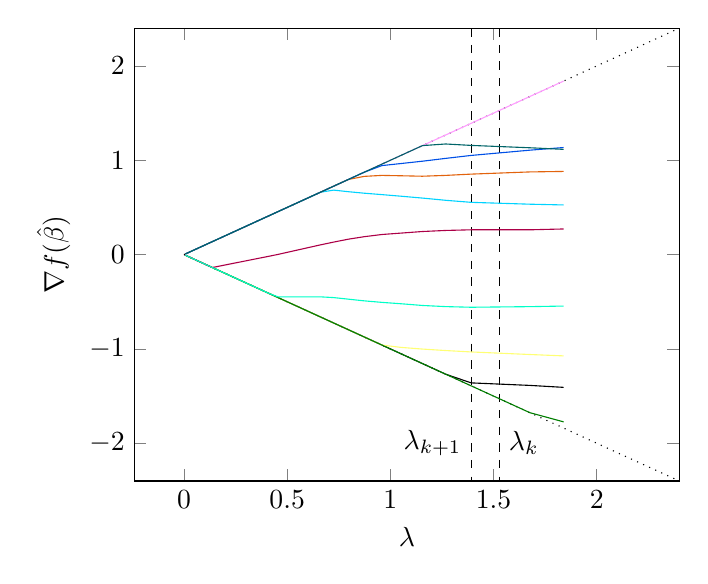
\begin{tikzpicture}
\begin{axis}[xlabel={$\lambda$}, ylabel={$\nabla f(\hat\beta)$}, width={8.5cm}, ymax={2.4}, ymin={-2.4}, xmax={2.4}]
    \draw[dashed] ({axis cs:1.3917299769873681,0}|-{rel axis cs:0,1}) -- ({axis cs:1.3917299769873681,0}|-{rel axis cs:0,0});
    \draw[dashed] ({axis cs:1.527421931643316,0}|-{rel axis cs:0,1}) -- ({axis cs:1.527421931643316,0}|-{rel axis cs:0,0});
    \addplot[dotted]
        coordinates {
            (0,0)
            (4,4)
        }
        ;
    \addplot[dotted]
        coordinates {
            (0,0)
            (4,-4)
        }
        ;
    \node 
    [left]  at 
    (1.3917299769873681,-2)
    {$\lambda_{k+1}$};
    \node 
    [right]  at 
    (1.527421931643316,-2)
    {$\lambda_{k}$};
    % \draw 
    % [decorate, decoration={brace}, xshift=2pt] (1.527421931643316,1.2560380223314203)
    % --
    % (1.527421931643316,-1.2560380223314203)
    % node [right,black,midway]{\footnotesize strong bound};]
    \addplot[color={rgb,1:red,0.0;green,0.0;blue,0.0}]
        table[row sep={\\}]
        {
            \\
            1.839785124133282  -1.4077202655506813  \\
            1.6763436843655586  -1.3869613211255392  \\
            1.527421931643316  -1.372974372747998  \\
            1.3917299769873681  -1.3602300019385394  \\
            1.268092521600357  -1.2680981590214144  \\
            1.1554386769908218  -1.155442990391262  \\
            1.0527926894493917  -1.0527950409055304  \\
            0.959265488536946  -0.9592563022504802  \\
            0.8740469863817951  -0.8740136245098727  \\
            0.796399061086074  -0.7963927481850348  \\
            0.7256491634669751  -0.7256503839758264  \\
            0.6611844917574681  -0.6612256935118651  \\
            0.6024466838105537  -0.6024557616294893  \\
            0.5489269808334608  -0.5489352473825738  \\
            0.5001618207623705  -0.5001693529404507  \\
            0.4557288231095828  -0.45573568614972415  \\
            0.4152431305057957  -0.4152556144961029  \\
            0.3783540752496846  -0.37836661263540705  \\
            0.34474214199202985  -0.3447535650486027  \\
            0.31411620024661524  -0.3141266085104193  \\
            0.28621098275723084  -0.2862204663795648  \\
            0.26078478787960124  -0.26083262949872155  \\
            0.2376173860773707  -0.23766098662087795  \\
            0.21650811239921539  -0.2165478395648333  \\
            0.19727412841503122  -0.19731032632873968  \\
            0.1797488385569208  -0.17978182074774082  \\
            0.16378044714808207  -0.16381049929197253  \\
            0.1492306436212737  -0.14925802601552787  \\
            0.13597340453884807  -0.13597917728258543  \\
            0.1238939020380232  -0.12390014056372889  \\
            0.11288750924686765  -0.1128931543493642  \\
            0.1028588940563887  -0.10286403758075523  \\
            0.09372119339941025  -0.09372587998707005  \\
            0.08539526088423945  -0.08539953112836769  \\
            0.07780898126648483  -0.07781287215389417  \\
            0.07089664582130879  -0.07090019105300449  \\
            0.06459838320588741  -0.06460161348897028  \\
            0.058859640882480906  -0.05886258419611779  \\
            0.05363071261044923  -0.05363339444821467  \\
            0.04886630791457465  -0.048868751505264686  \\
            0.044525159800631986  -0.044527386309459856  \\
            0.040569667320426425  -0.040571696032346366  \\
            0.03696556989036824  -0.036967418377112635  \\
            0.033681650542687666  -0.03368333481496441  \\
            0.030689465538994057  -0.03069100018516373  \\
            0.027963098004221153  -0.027986104494638068  \\
            0.02547893344705368  -0.025499746436454043  \\
            0.023215455222500556  -0.02323441457472633  \\
            0.021153058165009335  -0.021170333145097392  \\
            0.01927387877790116  -0.01928961909526972  \\
            0.01756164050830826  -0.017575982499248043  \\
            0.016001512767459578  -0.016014580655451995  \\
            0.014579982475215659  -0.014591889448055664  \\
            0.013284737016233032  -0.01329558620642299  \\
            0.01210455759398035  -0.012114442972015223  \\
            0.011029222058889811  -0.011038229247185241  \\
            0.010049416368987792  -0.01005762338350017  \\
            0.009156653916119027  -0.00916413184208162  \\
            0.0083432020190067  -0.008350015626636686  \\
            0.00760201494646646  -0.007608223251973829  \\
            0.006926672890653523  -0.006967160900731626  \\
        }
        ;
    \addplot[color={rgb,1:red,1.0;green,1.0;blue,0.4549}]
        table[row sep={\\}]
        {
            \\
            1.839785124133282  -1.0740166024012727  \\
            1.6763436843655586  -1.0594544869154927  \\
            1.527421931643316  -1.0451902642046422  \\
            1.3917299769873681  -1.0321932427787441  \\
            1.268092521600357  -1.0173512166391305  \\
            1.1554386769908218  -1.0016060767090929  \\
            1.0527926894493917  -0.9841837507773538  \\
            0.959265488536946  -0.9592622167171292  \\
            0.8740469863817951  -0.8740301158898205  \\
            0.796399061086074  -0.7963925883654892  \\
            0.7256491634669751  -0.7256482826596983  \\
            0.6611844917574681  -0.6612071636572264  \\
            0.6024466838105537  -0.6024283924821208  \\
            0.5489269808334608  -0.5489102878041107  \\
            0.5001618207623705  -0.5001466106971787  \\
            0.4557288231095828  -0.4557149642646659  \\
            0.4152431305057957  -0.4152434412422857  \\
            0.3783540752496846  -0.37835507617537856  \\
            0.34474214199202985  -0.3447430538877129  \\
            0.31411620024661524  -0.3141170311319773  \\
            0.28621098275723084  -0.28621173982902726  \\
            0.26078478787960124  -0.26077574467382625  \\
            0.2376173860773707  -0.23760916619742814  \\
            0.21650811239921539  -0.2165006227546474  \\
            0.19727412841503122  -0.1972673041298264  \\
            0.1797488385569208  -0.17974262052240483  \\
            0.16378044714808207  -0.16377478150661473  \\
            0.1492306436212737  -0.1492254812997791  \\
            0.13597340453884807  -0.1359712745522819  \\
            0.1238939020380232  -0.12387127117967824  \\
            0.11288750924686765  -0.11286684252948499  \\
            0.1028588940563887  -0.10284006317743971  \\
            0.09372119339941025  -0.09370403540352074  \\
            0.08539526088423945  -0.0853796271574143  \\
            0.07780898126648483  -0.07779473639686238  \\
            0.07089664582130879  -0.07088366642664293  \\
            0.06459838320588741  -0.064586556864871  \\
            0.058859640882480906  -0.058848865161005286  \\
            0.05363071261044923  -0.05362089417437037  \\
            0.04886630791457465  -0.048857361721296184  \\
            0.044525159800631986  -0.04451700836250741  \\
            0.040569667320426425  -0.04056224003359853  \\
            0.03696556989036824  -0.03695880242323147  \\
            0.033681650542687666  -0.033675484278679314  \\
            0.030689465538994057  -0.03068384706888505  \\
            0.027963098004221153  -0.027940863534424515  \\
            0.02547893344705368  -0.025458479653743024  \\
            0.023215455222500556  -0.02319681458390611  \\
            0.021153058165009335  -0.02113607343979051  \\
            0.01927387877790116  -0.019258402927784055  \\
            0.01756164050830826  -0.01754753949004626  \\
            0.016001512767459578  -0.015988664444795693  \\
            0.014579982475215659  -0.0145682755621255  \\
            0.013284737016233032  -0.013274070113036017  \\
            0.01210455759398035  -0.012094838309064118  \\
            0.011029222058889811  -0.01102036620845793  \\
            0.010049416368987792  -0.010041347247900375  \\
            0.009156653916119027  -0.00914930163350964  \\
            0.0083432020190067  -0.008336502892920351  \\
            0.00760201494646646  -0.007595910952278082  \\
            0.006926672890653523  -0.0069078250525788755  \\
        }
        ;
    \addplot[color={rgb,1:red,1.0;green,0.6078;blue,1.0}]
        table[row sep={\\}]
        {
            \\
            1.839785124133282  1.8397851241332814  \\
            1.6763436843655586  1.6763435737142731  \\
            1.527421931643316  1.5274217418527607  \\
            1.3917299769873681  1.391729804057265  \\
            1.268092521600357  1.2680914205021188  \\
            1.1554386769908218  1.1554371367955463  \\
            1.0527926894493917  1.0527919387552134  \\
            0.959265488536946  0.9592702558864394  \\
            0.8740469863817951  0.8740672706735734  \\
            0.796399061086074  0.7964046343401125  \\
            0.7256491634669751  0.7256483944132225  \\
            0.6611844917574681  0.6611605169065458  \\
            0.6024466838105537  0.6024664616368461  \\
            0.5489269808334608  0.5489449997288162  \\
            0.5001618207623705  0.5001782389043823  \\
            0.4557288231095828  0.4557437827091072  \\
            0.4152431305057957  0.4152372733166853  \\
            0.3783540752496846  0.37834810595204593  \\
            0.34474214199202985  0.34473670330304995  \\
            0.31411620024661524  0.31411124471572427  \\
            0.28621098275723084  0.2862064674620465  \\
            0.26078478787960124  0.26077418627403975  \\
            0.2376173860773707  0.2376077130814579  \\
            0.21650811239921539  0.21649929873953025  \\
            0.19727412841503122  0.19726609773659273  \\
            0.1797488385569208  0.17974152130182128  \\
            0.16378044714808207  0.16377377993775838  \\
            0.1492306436212737  0.14922456870753986  \\
            0.13597340453884807  0.1359975805661932  \\
            0.1238939020380232  0.12395417963980454  \\
            0.11288750924686765  0.11294254102291855  \\
            0.1028588940563887  0.10290903723355237  \\
            0.09372119339941025  0.09376688199557048  \\
            0.08539526088423945  0.08543689063144173  \\
            0.07780898126648483  0.07784691274168168  \\
            0.07089664582130879  0.07093120756879294  \\
            0.06459838320588741  0.06462987458298106  \\
            0.058859640882480906  0.05888833465242757  \\
            0.05363071261044923  0.05365685730495745  \\
            0.04886630791457465  0.04889012998648044  \\
            0.044525159800631986  0.044546865585326216  \\
            0.040569667320426425  0.040589444823032055  \\
            0.03696556989036824  0.0369835904141515  \\
            0.033681650542687666  0.033698070172804774  \\
            0.030689465538994057  0.030704426494426045  \\
            0.027963098004221153  0.02802531416566563  \\
            0.02547893344705368  0.0255363416101223  \\
            0.023215455222500556  0.02326777514724212  \\
            0.021153058165009335  0.021200730310042087  \\
            0.01927387877790116  0.01931731586357297  \\
            0.01756164050830826  0.01760121876304457  \\
            0.016001512767459578  0.01603757499912812  \\
            0.014579982475215659  0.014612841037614432  \\
            0.013284737016233032  0.013314676514510375  \\
            0.01210455759398035  0.012131837349747548  \\
            0.011029222058889811  0.011054078356340695  \\
            0.010049416368987792  0.010072064501480335  \\
            0.009156653916119027  0.009177290050941603  \\
            0.0083432020190067  0.008362004896487108  \\
            0.00760201494646646  0.007619147428134818  \\
            0.006926672890653523  0.006991613998442512  \\
        }
        ;
    \addplot[color={rgb,1:red,0.0;green,0.8275;blue,1.0}]
        table[row sep={\\}]
        {
            \\
            1.839785124133282  0.5262818345203535  \\
            1.6763436843655586  0.534233758654948  \\
            1.527421931643316  0.5445507732951834  \\
            1.3917299769873681  0.5539512511560487  \\
            1.268092521600357  0.5755617465578776  \\
            1.1554386769908218  0.5991746832820806  \\
            1.0527926894493917  0.618744458910842  \\
            0.959265488536946  0.6357746362395237  \\
            0.8740469863817951  0.6507163288487767  \\
            0.796399061086074  0.6667630765307442  \\
            0.7256491634669751  0.6834952403873034  \\
            0.6611844917574681  0.6611968292640323  \\
            0.6024466838105537  0.6024363329713686  \\
            0.5489269808334608  0.5489175474749682  \\
            0.5001618207623705  0.5001532254393263  \\
            0.4557288231095828  0.4557209913713487  \\
            0.4152431305057957  0.4152443377154589  \\
            0.3783540752496846  0.37835416163470703  \\
            0.34474214199202985  0.34474222067869875  \\
            0.31411620024661524  0.3141162719429976  \\
            0.28621098275723084  0.2862110480843047  \\
            0.26078478787960124  0.2607872837299235  \\
            0.2376173860773707  0.23761965606434202  \\
            0.21650811239921539  0.216510180722962  \\
            0.19727412841503122  0.1972760129945995  \\
            0.1797488385569208  0.17975055571563442  \\
            0.16378044714808207  0.1637820117591483  \\
            0.1492306436212737  0.14923206923660504  \\
            0.13597340453884807  0.13596883260158948  \\
            0.1238939020380232  0.12387996029846464  \\
            0.11288750924686765  0.11287478604400487  \\
            0.1028588940563887  0.10284730110868157  \\
            0.09372119339941025  0.09371063033712901  \\
            0.08539526088423945  0.08538563621529799  \\
            0.07780898126648483  0.07780021162660539  \\
            0.07089664582130879  0.07088865525206595  \\
            0.06459838320588741  0.0645911024967932  \\
            0.058859640882480906  0.05885300697151626  \\
            0.05363071261044923  0.053624668037850896  \\
            0.04886630791457465  0.04886080032514656  \\
            0.044525159800631986  0.044520141490269005  \\
            0.040569667320426425  0.04056509482292512  \\
            0.03696556989036824  0.03696140360094269  \\
            0.033681650542687666  0.033677854374931836  \\
            0.030689465538994057  0.03068600661231927  \\
            0.027963098004221153  0.02795465341355136  \\
            0.02547893344705368  0.02547105016933694  \\
            0.023215455222500556  0.023208269620523928  \\
            0.021153058165009335  0.02114651087569309  \\
            0.01927387877790116  0.01926791313120384  \\
            0.01756164050830826  0.017556204833213837  \\
            0.016001512767459578  0.015996559982759187  \\
            0.014579982475215659  0.014575469682257702  \\
            0.013284737016233032  0.013280625127363797  \\
            0.01210455759398035  0.01210081099398526  \\
            0.011029222058889811  0.011025808296512346  \\
            0.010049416368987792  0.010046305875851416  \\
            0.009156653916119027  0.009153819750619857  \\
            0.0083432020190067  0.008340619632959163  \\
            0.00760201494646646  0.007599661972478075  \\
            0.006926672890653523  0.006938247028719643  \\
        }
        ;
    \addplot[color={rgb,1:red,0.8863;green,0.3882;blue,0.051}]
        table[row sep={\\}]
        {
            \\
            1.839785124133282  0.8817437504727766  \\
            1.6763436843655586  0.8764029656563675  \\
            1.527421931643316  0.8642526181103705  \\
            1.3917299769873681  0.8531816704687174  \\
            1.268092521600357  0.8396096892176024  \\
            1.1554386769908218  0.8308134826424433  \\
            1.0527926894493917  0.8356460692390775  \\
            0.959265488536946  0.8395549699310465  \\
            0.8740469863817951  0.8294534875626539  \\
            0.796399061086074  0.7964048236049572  \\
            0.7256491634669751  0.7256489759532192  \\
            0.6611844917574681  0.6611630441550489  \\
            0.6024466838105537  0.6024671125855324  \\
            0.5489269808334608  0.5489455962588012  \\
            0.5001618207623705  0.500178782441049  \\
            0.4557288231095828  0.4557442779594743  \\
            0.4152431305057957  0.4152387874408213  \\
            0.3783540752496846  0.37835037867040106  \\
            0.34474214199202985  0.34473877402041775  \\
            0.31411620024661524  0.31411313147627523  \\
            0.28621098275723084  0.2862081866079899  \\
            0.26078478787960124  0.2607783531703273  \\
            0.2376173860773707  0.23761151617256815  \\
            0.21650811239921539  0.21650276397148918  \\
            0.19727412841503122  0.19726925512689003  \\
            0.1797488385569208  0.17974439819826646  \\
            0.16378044714808207  0.16377640125865256  \\
            0.1492306436212737  0.1492269571575102  \\
            0.13597340453884807  0.13599652652692876  \\
            0.1238939020380232  0.12395464551935445  \\
            0.11288750924686765  0.11294296080154165  \\
            0.1028588940563887  0.10290941970627922  \\
            0.09372119339941025  0.09376723049044494  \\
            0.08539526088423945  0.08543720816699153  \\
            0.07780898126648483  0.0778472020682489  \\
            0.07089664582130879  0.07093147119238505  \\
            0.06459838320588741  0.06463011478698018  \\
            0.058859640882480906  0.05888855351736519  \\
            0.05363071261044923  0.05365705672653711  \\
            0.04886630791457465  0.04889031169199658  \\
            0.044525159800631986  0.04454703114862497  \\
            0.040569667320426425  0.04058959567814366  \\
            0.03696556989036824  0.036983727867710724  \\
            0.033681650542687666  0.03369819541536849  \\
            0.030689465538994057  0.03070454061078536  \\
            0.027963098004221153  0.028023191776597366  \\
            0.02547893344705368  0.025534398359090122  \\
            0.023215455222500556  0.023266003958779074  \\
            0.021153058165009335  0.021199116458854465  \\
            0.01927387877790116  0.01931584538232567  \\
            0.01756164050830826  0.017599878915296418  \\
            0.016001512767459578  0.016036354179760792  \\
            0.014579982475215659  0.014611728672475106  \\
            0.013284737016233032  0.013313662968824183  \\
            0.01210455759398035  0.012130913844666491  \\
            0.011029222058889811  0.011053236892905912  \\
            0.010049416368987792  0.010071297791337593  \\
            0.009156653916119027  0.009176591453214976  \\
            0.0083432020190067  0.008361368360257462  \\
            0.00760201494646646  0.007618567440028876  \\
            0.006926672890653523  0.0069786583100767885  \\
        }
        ;
    \addplot[color={rgb,1:red,0.0;green,0.4941;blue,0.0}]
        table[row sep={\\}]
        {
            \\
            1.839785124133282  -1.7735789352411289  \\
            1.6763436843655586  -1.6763436843655581  \\
            1.527421931643316  -1.5274219316433155  \\
            1.3917299769873681  -1.391729976987368  \\
            1.268092521600357  -1.2680925216003567  \\
            1.1554386769908218  -1.1554387352256574  \\
            1.0527926894493917  -1.0527927253180733  \\
            0.959265488536946  -0.9592654218675132  \\
            0.8740469863817951  -0.8740488675653486  \\
            0.796399061086074  -0.796401157977832  \\
            0.7256491634669751  -0.7256498327295953  \\
            0.6611844917574681  -0.6611797549521219  \\
            0.6024466838105537  -0.602454516052506  \\
            0.5489269808334608  -0.5489341243907603  \\
            0.5001618207623705  -0.5001683297055934  \\
            0.4557288231095828  -0.45573475381622813  \\
            0.4152431305057957  -0.41524297572645497  \\
            0.3783540752496846  -0.3783537279901447  \\
            0.34474214199202985  -0.3447418256244353  \\
            0.31411620024661524  -0.3141159119842545  \\
            0.28621098275723084  -0.28621072010330356  \\
            0.26078478787960124  -0.26078846836502  \\
            0.2376173860773707  -0.23762073189963928  \\
            0.21650811239921539  -0.21651116098615403  \\
            0.19727412841503122  -0.19727690617391602  \\
            0.1797488385569208  -0.1797513695473617  \\
            0.16378044714808207  -0.16378275329230824  \\
            0.1492306436212737  -0.1492327448940026  \\
            0.13597340453884807  -0.1359688467753483  \\
            0.1238939020380232  -0.12388826866245196  \\
            0.11288750924686765  -0.11288236943386355  \\
            0.1028588940563887  -0.10285421083493197  \\
            0.09372119339941025  -0.09371692622240055  \\
            0.08539526088423945  -0.0853913727914745  \\
            0.07780898126648483  -0.07780543858116488  \\
            0.07089664582130879  -0.07089341785838886  \\
            0.06459838320588741  -0.06459544200629642  \\
            0.058859640882480906  -0.05885696097095554  \\
            0.05363071261044923  -0.05362827077487783  \\
            0.04886630791457465  -0.04886408300494525  \\
            0.044525159800631986  -0.04452313254584203  \\
            0.040569667320426425  -0.0405678201613648  \\
            0.03696556989036824  -0.036963886827826836  \\
            0.033681650542687666  -0.03368011699878376  \\
            0.030689465538994057  -0.030688068230903993  \\
            0.027963098004221153  -0.02795481245972661  \\
            0.02547893344705368  -0.02547131917080111  \\
            0.023215455222500556  -0.023208516846951927  \\
            0.021153058165009335  -0.021146736171030956  \\
            0.01927387877790116  -0.019268118412388815  \\
            0.01756164050830826  -0.017556391877790754  \\
            0.016001512767459578  -0.015996730410811653  \\
            0.014579982475215659  -0.014575624969951538  \\
            0.013284737016233032  -0.013280766619727026  \\
            0.01210455759398035  -0.012100939916557136  \\
            0.011029222058889811  -0.011025925765957846  \\
            0.010049416368987792  -0.010046412909635379  \\
            0.009156653916119027  -0.009153917275817458  \\
            0.0083432020190067  -0.008340708494287197  \\
            0.00760201494646646  -0.007599742939610854  \\
            0.006926672890653523  -0.006909246075506272  \\
        }
        ;
    \addplot[color={rgb,1:red,0.0;green,0.3137;blue,0.902}]
        table[row sep={\\}]
        {
            \\
            1.839785124133282  1.135089754174434  \\
            1.6763436843655586  1.1071139623655615  \\
            1.527421931643316  1.0779239477935385  \\
            1.3917299769873681  1.051327105647608  \\
            1.268092521600357  1.0200279843113864  \\
            1.1554386769908218  0.9900664325473005  \\
            1.0527926894493917  0.9656388790664223  \\
            0.959265488536946  0.9437444131949158  \\
            0.8740469863817951  0.8740485689218533  \\
            0.796399061086074  0.7963995354471453  \\
            0.7256491634669751  0.7256491217992942  \\
            0.6611844917574681  0.6611835673153322  \\
            0.6024466838105537  0.6024491755659228  \\
            0.5489269808334608  0.5489292509956886  \\
            0.5001618207623705  0.5001638892494293  \\
            0.4557288231095828  0.455730707837952  \\
            0.4152431305057957  0.41524492767887466  \\
            0.3783540752496846  0.37835699281762414  \\
            0.34474214199202985  0.3447448002387928  \\
            0.31411620024661524  0.31411862234205856  \\
            0.28621098275723084  0.28621318968039045  \\
            0.26078478787960124  0.26078947152604376  \\
            0.2376173860773707  0.2376216655364002  \\
            0.21650811239921539  0.21651201168186554  \\
            0.19727412841503122  0.19727768129614762  \\
            0.1797488385569208  0.17975207580987074  \\
            0.16378044714808207  0.16378339681240223  \\
            0.1492306436212737  0.1492333312455451  \\
            0.13597340453884807  0.13598458950805786  \\
            0.1238939020380232  0.12391877366999463  \\
            0.11288750924686765  0.11291019881807988  \\
            0.1028588940563887  0.1028795680134583  \\
            0.09372119339941025  0.09374003073928097  \\
            0.08539526088423945  0.0854124247667541  \\
            0.07780898126648483  0.07782462035698239  \\
            0.07089664582130879  0.07091089557810949  \\
            0.06459838320588741  0.06461136705356804  \\
            0.058859640882480906  0.05887147128091845  \\
            0.05363071261044923  0.05364149202889543  \\
            0.04886630791457465  0.04887612971919543  \\
            0.044525159800631986  0.04453410906320032  \\
            0.040569667320426425  0.04057782155517334  \\
            0.03696556989036824  0.03697299972537414  \\
            0.033681650542687666  0.033688420331629006  \\
            0.030689465538994057  0.030695633918544067  \\
            0.027963098004221153  0.02798984504654397  \\
            0.02547893344705368  0.02550355258227658  \\
            0.023215455222500556  0.023237889904029186  \\
            0.021153058165009335  0.02117349984475035  \\
            0.01927387877790116  0.019292504475629687  \\
            0.01756164050830826  0.017578611550392052  \\
            0.016001512767459578  0.01601697614893885  \\
            0.014579982475215659  0.014594072132502944  \\
            0.013284737016233032  0.013297574987199634  \\
            0.01210455759398035  0.012116255074989191  \\
            0.011029222058889811  0.011039880367925416  \\
            0.010049416368987792  0.01005912782322409  \\
            0.009156653916119027  0.009165502631526783  \\
            0.0083432020190067  0.008351264638925694  \\
            0.00760201494646646  0.007609361305453279  \\
            0.006926672890653523  0.006948687748096627  \\
        }
        ;
    \addplot[color={rgb,1:red,0.6745;green,0.0;blue,0.2784}]
        table[row sep={\\}]
        {
            \\
            1.839785124133282  0.27166717270336277  \\
            1.6763436843655586  0.26282311169114886  \\
            1.527421931643316  0.26284489047542386  \\
            1.3917299769873681  0.2628647463964542  \\
            1.268092521600357  0.2558751900981948  \\
            1.1554386769908218  0.24463973790676177  \\
            1.0527926894493917  0.2280796660946305  \\
            0.959265488536946  0.21294150755378927  \\
            0.8740469863817951  0.18996460284401231  \\
            0.796399061086074  0.16333980815528096  \\
            0.7256491634669751  0.13272353146394295  \\
            0.6611844917574681  0.10302551991449099  \\
            0.6024466838105537  0.07413244085917409  \\
            0.5489269808334608  0.04779948346551989  \\
            0.5001618207623705  0.023805875011035642  \\
            0.4557288231095828  0.001943792602986445  \\
            0.4152431305057957  -0.01610576196058167  \\
            0.3783540752496846  -0.03217249429607616  \\
            0.34474214199202985  -0.04681218681148503  \\
            0.31411620024661524  -0.06015132938878707  \\
            0.28621098275723084  -0.07230545930373283  \\
            0.26078478787960124  -0.08337787969527607  \\
            0.2376173860773707  -0.09346862584109146  \\
            0.21650811239921539  -0.10266293896436345  \\
            0.19727412841503122  -0.11104045465152161  \\
            0.1797488385569208  -0.11867373493443248  \\
            0.16378044714808207  -0.1256288956352116  \\
            0.1492306436212737  -0.1319661790285596  \\
            0.13597340453884807  -0.13597721900505028  \\
            0.1238939020380232  -0.12390210787111552  \\
            0.11288750924686765  -0.1128949956999519  \\
            0.1028588940563887  -0.10286571545449083  \\
            0.09372119339941025  -0.09372740880335872  \\
            0.08539526088423945  -0.08540092412883162  \\
            0.07780898126648483  -0.077814141404036  \\
            0.07089664582130879  -0.07090134754646193  \\
            0.06459838320588741  -0.06460266724273649  \\
            0.058859640882480906  -0.05886354433730366  \\
            0.05363071261044923  -0.05363426929310386  \\
            0.04886630791457465  -0.04886954863134488  \\
            0.044525159800631986  -0.044528112621056194  \\
            0.040569667320426425  -0.04057235782042237  \\
            0.03696556989036824  -0.036968021373760054  \\
            0.033681650542687666  -0.0336838842430515  \\
            0.030689465538994057  -0.030691500803573968  \\
            0.027963098004221153  -0.02797089594992417  \\
            0.02547893344705368  -0.025486130402715287  \\
            0.023215455222500556  -0.02322201391048899  \\
            0.021153058165009335  -0.02115903421129019  \\
            0.01927387877790116  -0.019279323928899236  \\
            0.01756164050830826  -0.017566601927102063  \\
            0.016001512767459578  -0.016006033427482063  \\
            0.014579982475215659  -0.014584101532261178  \\
            0.013284737016233032  -0.013288490147603306  \\
            0.01210455759398035  -0.012107977307503735  \\
            0.011029222058889811  -0.011032337974488993  \\
            0.010049416368987792  -0.010052255475232856  \\
            0.009156653916119027  -0.009159240803990283  \\
            0.0083432020190067  -0.008345559094889304  \\
            0.00760201494646646  -0.00760416262622404  \\
            0.006926672890653523  -0.006930576992560517  \\
        }
        ;
    \addplot[color={rgb,1:red,0.0;green,1.0;blue,0.7843}]
        table[row sep={\\}]
        {
            \\
            1.839785124133282  -0.5457122136864775  \\
            1.6763436843655586  -0.5519040341475189  \\
            1.527421931643316  -0.5552602552360572  \\
            1.3917299769873681  -0.5583183135173444  \\
            1.268092521600357  -0.551557927335853  \\
            1.1554386769908218  -0.5394217331984487  \\
            1.0527926894493917  -0.5214957209340106  \\
            0.959265488536946  -0.5066338186587006  \\
            0.8740469863817951  -0.4906790683791963  \\
            0.796399061086074  -0.47262329580902657  \\
            0.7256491634669751  -0.45594919886022495  \\
            0.6611844917574681  -0.44797798297355074  \\
            0.6024466838105537  -0.44810656671413673  \\
            0.5489269808334608  -0.4482192285223354  \\
            0.5001618207623705  -0.4483218778597154  \\
            0.4557288231095828  -0.4484154081125965  \\
            0.4152431305057957  -0.4152433406358467  \\
            0.3783540752496846  -0.3783537243458599  \\
            0.34474214199202985  -0.3447418222699672  \\
            0.31411620024661524  -0.31411590892779007  \\
            0.28621098275723084  -0.28621071731836717  \\
            0.26078478787960124  -0.2607844443394749  \\
            0.2376173860773707  -0.23761706965357263  \\
            0.21650811239921539  -0.2165078240838153  \\
            0.19727412841503122  -0.19727386571277947  \\
            0.1797488385569208  -0.17974859919241318  \\
            0.16378044714808207  -0.16378022904805767  \\
            0.1492306436212737  -0.14923044489665452  \\
            0.13597340453884807  -0.13596704132892784  \\
            0.1238939020380232  -0.12387984433101144  \\
            0.11288750924686765  -0.11287468245352944  \\
            0.1028588940563887  -0.10284720672005845  \\
            0.09372119339941025  -0.0937105443337278  \\
            0.08539526088423945  -0.08538555785220199  \\
            0.07780898126648483  -0.07780014022507103  \\
            0.07089664582130879  -0.07088859019364735  \\
            0.06459838320588741  -0.06459104321798524  \\
            0.058859640882480906  -0.05885295295887438  \\
            0.05363071261044923  -0.053624618823543226  \\
            0.04886630791457465  -0.04886075548290233  \\
            0.044525159800631986  -0.04452010063168643  \\
            0.040569667320426425  -0.0405650575941064  \\
            0.03696556989036824  -0.036961369679429854  \\
            0.033681650542687666  -0.03367782346691275  \\
            0.030689465538994057  -0.030685978450083095  \\
            0.027963098004221153  -0.027949930887841427  \\
            0.02547893344705368  -0.025466775773739327  \\
            0.023215455222500556  -0.023204375570947157  \\
            0.021153058165009335  -0.021142962771972983  \\
            0.01927387877790116  -0.019264680231371355  \\
            0.01756164050830826  -0.017553259135294503  \\
            0.016001512767459578  -0.015993875972524253  \\
            0.014579982475215659  -0.014573024112094744  \\
            0.013284737016233032  -0.013278396814913744  \\
            0.01210455759398035  -0.012098780638671975  \\
            0.011029222058889811  -0.01102395831236918  \\
            0.010049416368987792  -0.01004462023920063  \\
            0.009156653916119027  -0.009152283861283585  \\
            0.0083432020190067  -0.008339220187798731  \\
            0.00760201494646646  -0.0075983868501685505  \\
            0.006926672890653523  -0.00691964342724483  \\
        }
        ;
    \addplot[color={rgb,1:red,0.0;green,0.3922;blue,0.4078}]
        table[row sep={\\}]
        {
            \\
            1.839785124133282  1.1157355634468402  \\
            1.6763436843655586  1.1325274950490352  \\
            1.527421931643316  1.1456001545954875  \\
            1.3917299769873681  1.157511464002459  \\
            1.268092521600357  1.1726662727727077  \\
            1.1554386769908218  1.155438676990822  \\
            1.0527926894493917  1.0527926894493917  \\
            0.959265488536946  0.9592654885369458  \\
            0.8740469863817951  0.8740469863817953  \\
            0.796399061086074  0.7963990610860745  \\
            0.7256491634669751  0.7256491634669753  \\
            0.6611844917574681  0.6611844917574682  \\
            0.6024466838105537  0.6024466838105534  \\
            0.5489269808334608  0.5489269808334606  \\
            0.5001618207623705  0.5001618207623703  \\
            0.4557288231095828  0.4557288231095826  \\
            0.4152431305057957  0.4152431305057954  \\
            0.3783540752496846  0.3783540752496847  \\
            0.34474214199202985  0.34474214199202957  \\
            0.31411620024661524  0.3141162002466153  \\
            0.28621098275723084  0.286210982757231  \\
            0.26078478787960124  0.2607847878796014  \\
            0.2376173860773707  0.2376173860773704  \\
            0.21650811239921539  0.21650811239921566  \\
            0.19727412841503122  0.1972741284150313  \\
            0.1797488385569208  0.17974883855692073  \\
            0.16378044714808207  0.16378044714808232  \\
            0.1492306436212737  0.1492306436212739  \\
            0.13597340453884807  0.13597340453884837  \\
            0.1238939020380232  0.1238939020380234  \\
            0.11288750924686765  0.11288750924686786  \\
            0.1028588940563887  0.10285889405638869  \\
            0.09372119339941025  0.0937211933994106  \\
            0.08539526088423945  0.08539526088423952  \\
            0.07780898126648483  0.07780898126648492  \\
            0.07089664582130879  0.0708966458213087  \\
            0.06459838320588741  0.06459838320588732  \\
            0.058859640882480906  0.058859640882480996  \\
            0.05363071261044923  0.053630712610449466  \\
            0.04886630791457465  0.04886630791457489  \\
            0.044525159800631986  0.044525159800631896  \\
            0.040569667320426425  0.04056966732042648  \\
            0.03696556989036824  0.036965569890368276  \\
            0.033681650542687666  0.03368165054268768  \\
            0.030689465538994057  0.03068946553899421  \\
            0.027963098004221153  0.027963098004221205  \\
            0.02547893344705368  0.025478933447053688  \\
            0.023215455222500556  0.023215455222500833  \\
            0.021153058165009335  0.021153058165009654  \\
            0.01927387877790116  0.01927387877790155  \\
            0.01756164050830826  0.017561640508308246  \\
            0.016001512767459578  0.016001512767459588  \\
            0.014579982475215659  0.014579982475215983  \\
            0.013284737016233032  0.013284737016233308  \\
            0.01210455759398035  0.012104557593980486  \\
            0.011029222058889811  0.011029222058889772  \\
            0.010049416368987792  0.01004941636898815  \\
            0.009156653916119027  0.009156653916119119  \\
            0.0083432020190067  0.00834320201900672  \\
            0.00760201494646646  0.007602014946466475  \\
            0.006926672890653523  0.006926672890653485  \\
        }
        ;
\end{axis}
\end{tikzpicture}

    \caption{The gradient vector along the lasso path}
  \end{figure}
\end{frame}

\begin{frame}{Screening Rules as a Gradient Estimate}
  From now on, let \(c(\lambda) \coloneqq -\nabla f(\beta(\lambda))\)
  be the so-called \alert{correlation} vector.

  \medskip

  Now note that the stationarity criterion, \(\boldsymbol{0} \in \nabla f(\beta)
  + \lambda \partial\), suggests a simple template for a screening rule:
  substitute the true gradient (correlation) vector in the optimality condition
  with some estimate. If this estimate is \(\tilde c\), simply input this into
  the optimality condition, that is, check if
  \[
    |\tilde c_j| < \lambda,
  \]
  and discard any predictors that fail this test. \medskip

  If the gradient estimate is accurate enough and not too conservative, we
  probably have a useful rule.
\end{frame}

\begin{frame}{The Strong Rule}
  The Strong Rule gradient estimate is
  \[
    \tilde c^S(\lambda_{k+1}) =
    \underbrace{c(\lambda_k)}_\text{previous gradient} +
    \underbrace{(\lambda_k - \lambda_{k+1})\sign(c(\lambda_k))}_\text{unit
      slope
      bound}.
  \]
  \begin{columns}
    \begin{column}{0.45\linewidth}
      simple idea: assume that the slope of the gradient is bounded by one (the
      unit slope bound) \medskip

      discovered by \parencite{tibshirani2012}
    \end{column}
    \begin{column}{0.45\linewidth}
      \begin{figure}
        \centering
        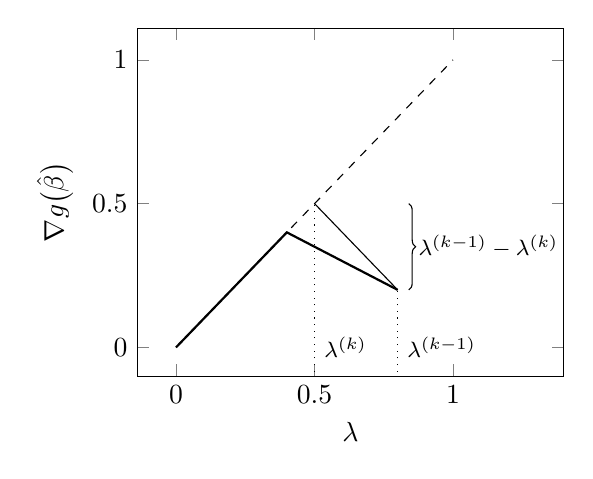
\begin{tikzpicture}
\begin{axis}[
    ylabel = \(\nabla g\big(\hat\beta\big)\),
    xlabel = \(\lambda\),
    xmax = 1.4,
    ymin = -0.1,
    width = 7cm,
    height = 6cm
]
\addplot[style = dashed]
    coordinates {
        (0,0)
        (1,1)
    };
\addplot[]
    coordinates {
        (0.8,0.2)
        (0.5,0.5)
    };
\addplot[thick]
    coordinates {
        (0.8,0.2)
        (0.4,0.4)
        (0,0)
    };
\draw [decorate,decoration={brace},xshift=4pt]
(0.8,0.5) -- (0.8,0.2)node [right,black,midway] {\footnotesize
$\lambda^{(k-1)}-\lambda^{(k)}$};

\addplot[style=dotted]
    coordinates {
        (0.5,-0.2)
        (0.5,0.5)
    };
\addplot[style=dotted]
    coordinates {
        (0.8,-0.2)
        (0.8,0.2)
    };
\node [right] at (0.5,0) {\footnotesize$\lambda^{(k)}$};
\node [right] at (0.8,0) {\footnotesize$\lambda^{(k-1)}$};
\end{axis}
\end{tikzpicture}
        \caption{The unit slope bound}
      \end{figure}
    \end{column}
  \end{columns}
\end{frame}

\begin{frame}{The Working Set Algorithm}
  The Strong Rule turns out to be very conservative when predictors are
  correlated. \medskip

  It turns out that a better alternative is to use the predictors that have
  \alert{ever been active} as a screened set and then
  \begin{enumerate}
    \item fit the lasso on the predictors in the screened set,
    \item check the optimality conditions in the strong set, and then
    \item check the optimality conditions for all predictors.
  \end{enumerate}
  Whenever we encounter violations (in step 2 or 3), go back to step 1 and
  repeat.

  \medskip

  This method is called the \alert{working set strategy} and is used in many
  popular implementations, such as \texttt{glmnet}~\parencite{friedman2010}
\end{frame}

\section{The Hessian Screening Rule}

\begin{frame}{The Ordinary Lasso}
  We now focus on the ordinary lasso: \(\ell_1\)-regularized least
  squares, where we have
  \[
    f(\beta) = \frac 1 2 \lVert y - X\beta \rVert_2^2
  \]
  and
  \[
    \nabla f(\beta) = X^T(X\beta - y).
  \]
  \pause
  It turns out that we can express the solution as a function of
  \(\lambda\):
  \begin{equation*}
    \label{eq:solution}
    \hat\beta(\lambda) = \big({X_\mathcal{A}}^TX_\mathcal{A}\big)^{-1}
    \big({X_\mathcal{A}}^Ty - \lambda \sign(\hat\beta_\mathcal{A})\big).
  \end{equation*}
  \pause
  This function is piece-wise linear
  for an interval \([\lambda_k,\lambda_{k+1}]\) in which no changes occur in
  the active set, which means we can retrieve any solution in this range via
  \begin{equation*}
    \hat\beta(\lambda_{k+1})_\mathcal{A} =
    \hat\beta(\lambda_k)_\mathcal{A} -
    (\lambda_k - \lambda_{k+1})\big({X_\mathcal{A}}^TX_\mathcal{A}\big)^{-1}
    \sign\big(\hat\beta(\lambda_k)_\mathcal{A}\big).
  \end{equation*}
\end{frame}

\begin{frame}{The Hessian Screening Rule}
  Now, we take this expression and stick it into the gradient at step \(k +
  1\):
  \begin{equation*}
    \begin{aligned}
      \tilde c^H(\lambda_{k+1})
       & = -\nabla f\big(\hat\beta(\lambda_{k+1})_\mathcal{A}\big)       \\
       & = c(\lambda_k) + (\lambda_{k+1} - \lambda_k)X^T {X_\mathcal{A}}
      \big({X_\mathcal{A}}^T{X_\mathcal{A}}\big)^{-1}
      \sign\big(\hat\beta(\lambda_k)_\mathcal{A}\big),
    \end{aligned}
  \end{equation*}
  which is the basic form of our screening rule: \alert{The Hessian Screening
    Rule}. \medskip

  Note that this is an exact expression for the correlation vector (negative
  gradient) at step \(k+1\) if the activate set has remained unchanged.\medskip

  The Hessian Screening Rule is a heuristic (un-safe) rule: it may result in
  violations.
\end{frame}

\begin{frame}{The Hessian and Strong Screening Rules}
  \begin{figure}
    \input{figures/estimate-comp.tikz}
    \caption{Conceptual comparison of screening rules}
  \end{figure}
\end{frame}

\begin{frame}{Tweaks}
  \begin{block}{Avoiding Expensive Inner Products}
    The expression
    \begin{equation*}
      \hat c^H(\lambda_{k+1})
      = c(\lambda_k) + (\lambda_{k+1} - \lambda_k)X^T {X_\mathcal{A}}
      \big({X_\mathcal{A}}^T{X_\mathcal{A}}\big)^{-1}
      \sign\big(\hat\beta(\lambda_k)_\mathcal{A}\big),
    \end{equation*}
    involves an expensive inner product with the full design matrix. Instead,
    we replace \(X\) with the columns indexed by the strong rule.
  \end{block}

  \begin{block}{Upwards Shift}
    We need some upwards bias on the estimate or else risk excessive numbers of
    violations. We add a fraction \(\gamma\) of the unit bound\footnote{We've
      set \(\gamma = 0.01\) in our simulations, which has worked very well.}
  \end{block}

\end{frame}

\begin{frame}{Warm Starts}
  The availability of the Hessian (and its inverse) enables a much improved
  warm
  start:
  \[
    \hat\beta(\lambda_{k+1})_\mathcal{A} \coloneqq
    \hat\beta(\lambda_k)_\mathcal{A} +
    (\lambda_k - \lambda_{k+1}) \big({X_\mathcal{A}}^T{X_\mathcal{A}}\big)^{-1}
    \sign\big(\hat\beta(\lambda_k)_\mathcal{A}\big)
  \]
  \pause
  \begin{figure}
    \centering
    \includegraphics{figures/hessian-warm-starts}
    \caption{Number of passes of coordinate descent for two datasets
      using either Hessian warm
      starts or standard warm starts.}
  \end{figure}

\end{frame}

\begin{frame}{Updating the Hessian}
  A potential hurdle with the screening rule is of course computing the Hessian
  and its inverse, which is an \(\mathcal{O}(|\mathcal{A}|^3 +
  |\mathcal{A}|^2n)\) operation if executed naively.

  \medskip

  Fortunately, we can compute these operations efficiently by sweeping columns
  of the Hessian (and inverse) in our out as we proceed along the path, with
  numerical complexity
  \begin{itemize}
    \item \(\mathcal{O}(|\mathcal{D}|^2n + n|\mathcal{D}||\mathcal{E}| +
          |\mathcal{D}^2||\mathcal{E}| + |\mathcal{D}|^3)\) when
          augmenting the Hessian and
    \item \(\mathcal{O}(|\mathcal{C}|^3 + |\mathcal{C}|^2|\mathcal{E}| +
          |\mathcal{C}||\mathcal{E}|^2)\) when reducing it,
  \end{itemize}
  where \(\mathcal{C} = \mathcal{A}_{k-1} \setminus \mathcal{A}_k\),
  \(\mathcal{D} = \mathcal{A}_k \setminus \mathcal{A}_{k-1}\), and
  \(\mathcal{E} = \mathcal{A}_k \cap \mathcal{A}_{k-1}\).
\end{frame}

\begin{frame}{General Loss Functions}

  The rule can be extended to many other loss functions in the family of
  generalized linear models.

  \medskip

  We skip the details here, but note the following:
  \begin{itemize}
    \item The gradient estimate is a natural extension of that in the ordinary
          lasso case, but now involves a matrix of weights---for logistic
          regression a diagonal matrix.
    \item The lasso path is no longer piece-wise linear, which means that our
          estimate is never exact.
    \item There is no longer any cheap way to update the Hessian. In our
          implementation, we decide heuristically whether to approximate it
          with an
          upper bound or compute it fully.
  \end{itemize}
\end{frame}

\subsection{Results}

\begin{frame}{Setup}
  The setup is as follows:
  \begin{itemize}
    \item We draw the rows of the predictor matrix i.i.d. from
          \(\mathcal{N}(0,\Sigma)\)
    \item The response is generated from \(\mathcal{N}(X\beta,\sigma^2 I)\)
          with
          \(\sigma^2 = \beta^T\Sigma \beta/\text{SNR}\) where SNR is the
          signal-to-noise ratio.
    \item We set \(s\) coefficients, equally spaced throughout the coefficient
          vector, to 1 and the rest to zero.
  \end{itemize}

  \begin{block}{Scenario 1 (Low-Dimensional)}
    \(n = 10\,000\), \(p = 100\), \(s = 5\), and \(\text{SNR} = 1\)
  \end{block}

  \begin{block}{Scenario 2 (High-Dimensional)}
    \(n = 400\), \(p = 40\,000\), \(s = 20\), and \(\text{SNR} = 2\)
  \end{block}

  \medskip

  Code is located at

  \href{https://github.com/jolars/HessianScreening}{\nolinkurl{github.com/jolars/HessianScreening}}
\end{frame}

\begin{frame}{Simulated Data}

  \begin{figure}
    \centering
    \includegraphics{figures/simulateddata-timings}
    \caption{Time to fit a full regularization path for
      \(\ell_1\)-regularized least-squares and logistic regression to
      a design with \(n\) observations, \(p\) predictors, and pairwise
      correlation between predictors of \(\rho\). Time is relative to the
      minimal value for each group.}
  \end{figure}

\end{frame}

\begin{frame}{Real Data: Least-Squares Regression}
  \begin{table}
    \caption{Time to fit a full regularization path of \(\ell_1\)-regularized
      least-squares regression to real data sets.}
    \csvreader[
      tabular={
          l
          S[table-format=6.0,round-mode=off]
          S[table-format=7.0,round-mode=off]
          S[table-format=0.4,round-precision=2]
          S[table-format=5.2]
          S[table-format=3.3]
          S[table-format=3.2]
          S[table-format=3.2]
        },
      before reading=\notsotiny\centering\sisetup{round-mode=figures,
        round-precision=3},
      table head=\toprule & & & & \multicolumn{4}{c}{Time (s)} \\
      \cmidrule(lr){5-8} Dataset & {\(n\)} & {\(p\)} & {Density} & {Gap Safe}
      &
      {Hessian} & {Working} & {EDPP} \\\midrule,
      table foot=\bottomrule
    ]%
    {tables/realdata-timings-gaussian.csv}%
    {dataset=\dataset, n=\n, p=\p, density=\density, GapSafe=\gapsafe,
      Hessian=\hessian, Working=\working,
      EDPP=\edpp}%
    {\dataset & \n & \p & \density & \gapsafe & \hessian & \working & \edpp}
  \end{table}
\end{frame}

\begin{frame}{Real Data: Logistic Regression}

  \begin{table}
    \caption{Time to fit a full regularization path of \(\ell_1\)-regularized
      logistic regression to real data sets.}
    \csvreader[
      tabular={
          l
          S[table-format=5.0,round-mode=off]
          S[table-format=7.0,round-mode=off]
          S[table-format=1.5,scientific-notation=fixed]
          S[table-format=5.2]
          S[table-format=4.2]
          S[table-format=4.2]
        },
      before reading=\scriptsize\centering\sisetup{round-mode=figures,
        round-precision=2},
      table head=\toprule & & & & \multicolumn{3}{c}{Time (s)} \\
      \cmidrule(lr){5-7} Dataset & {\(n\)} & {\(p\)} & {Density} & {Gap Safe}
      &
      {Hessian} & {Working}\\\midrule,
      table foot=\bottomrule
    ]%
    {tables/realdata-timings-binomial.csv}%
    {dataset=\dataset, n=\n, p=\p, density=\density, GapSafe=\gapsafe,
      Hessian=\hessian, Working=\working}%
    {\dataset & \n & \p & \density & \gapsafe & \hessian & \working}
  \end{table}

\end{frame}

\begin{frame}{Discussion}
  \begin{itemize}
    \item simple, intuitive, idea
    \item performs well in our examples
    \item handles the highly-correlated case very well
    \item works for arbitrary loss functions that are twice differentiable
    \item works for other penalty functions too (SLOPE, lasso variations)
    \item a paper is submitted and under review, but a pre-print is
      available~\parencite{larsson2021}.
  \end{itemize}
\end{frame}

\section{Adaptive Lasso Path (Work in Progress)}

\begin{frame}{Standard Grid Setup}
  The dominating choice for constructing the lasso path in the high-dimensional
  regime is to setup a log-spaced grid from \(\lambda_\text{min}\) to
  \(\lambda_\text{max}\) where
  \[
    \lambda_\text{min} =\lambda_\text{max} \times
    \begin{cases}
      10^{-2} & \text{if } p > n  \\
      10^{-4} & \text{otherwise.}
    \end{cases}
  \]
  Why this particular choice? We don't know.

  \begin{block}{Why Not Use LARS?}
    Homotopy methods scale poorly with \(p\), in the worst case requiring
    \((3^p
    + 1)/2\) steps
  \end{block}
\end{frame}

\begin{frame}{The Problem with the Heuristic}
  \begin{columns}[c]
    \begin{column}{0.45\linewidth}
      If the \(\lambda\) values are not spaced densely enough around critical
      points, the interpolated values doesn't capture the path accurately.

      \medskip

      On the other hand, if the values are spaced too densely where there are
      no critical points, then we are \alert{wasting} resources.
    \end{column}
    \begin{column}{0.45\linewidth}
      \begin{figure}
        \centering
        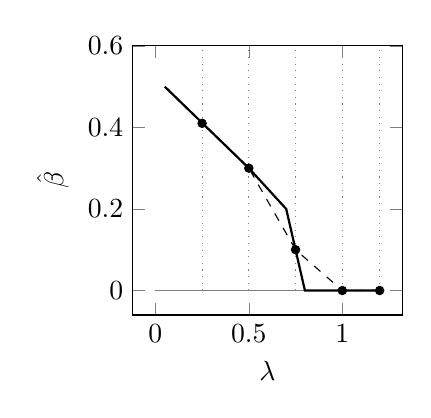
\begin{tikzpicture}
    \begin{axis}[
            ylabel = \(\hat\beta\),
            xlabel = \(\lambda\),
            % xmax = 1.4,
            % ymin = -0.1,
            ymax = 0.6,
            width = 5cm,
            height = 5cm
        ]
        \addplot[color = gray]
        coordinates {
                (0,0)
                (1.2,0)
            };
        \addplot[dotted, color = gray]
            coordinates {
                (1.2,0)
                (1.2,0.6)
            };
        \addplot[dotted, color = gray]
            coordinates {
                (1,0)
                (1,0.6)
            };
        \addplot[dotted, color = gray]
            coordinates {
                (0.75,0)
                (0.75,0.6)
            };
        \addplot[dotted, color = gray]
            coordinates {
                (0.5,0)
                (0.5,0.6)
            };
        \addplot[dotted, color = gray]
            coordinates {
                (0.25,0)
                (0.25,0.6)
            };
        \addplot[thick]
        coordinates {
                (1.2,0)
                (1,0)
                (0.8,0)
                (0.7, 0.2)
                (0.5, 0.3)
                (0.05, 0.5)
            };
        \addplot[mark=*, mark options = {style = solid, scale = 0.75}, solid, style = dashed]
        coordinates {
                (1.2,0)
                (1,0)
                (0.75, 0.1)
                (0.5, 0.3)
                (0.25, 0.41)
            };

        % \node [right] at (0.5,0) {\footnotesize\(\lambda_{k + 1}\)};
        % \node [right] at (0.8,0) {\footnotesize\(\lambda_{k}\)};
    \end{axis}
\end{tikzpicture}

        \caption{The exact path of a coefficient and the interpolated path
          based
          on the grid method as a dashed line.}
      \end{figure}
    \end{column}
  \end{columns}
\end{frame}

\begin{frame}{Lasso Path Profiles}
  When and how predictors enter the models along the lasso path vary greatly.
  \begin{figure}
    \includegraphics{figures/grid-paths.pdf}
    \caption{The number of included predictors at each step along the path for
      the
      standard grid path for the lasso. The number of included predictors
      varies
      considerably from data set to data set.\label{fig:grid-paths}}
  \end{figure}
\end{frame}

\begin{frame}{The Adaptive Lasso Path}
  The gradient estimate from the Hessian screening rule can be used to predict
  at which \(\lambda\) values the predictors will enter the model. \medskip

  With the Adaptive Lasso Path, we use this information to find the next
  \(\lambda\) at which a desired number of predictors will enter the model
  \medskip

  This lets us decide the resolution of the lasso path arbitrarily.
  %   \begin{equation*}
  %   \hat\lambda_j =
  %   \begin{cases}
  %     \max
  %     \left\{
  %       \splitfrac{\frac{c(\lambda)_j - \lambda \nabla c(\lambda)_j}
  %         {1 - \nabla c(\lambda)_j},}{\frac{\lambda \nabla c(\lambda)_j -
  %           c(\lambda)_j}{1 + \nabla c(\lambda)_j}}
  %     \right\}
  %      & \text{if } \hat\beta(\lambda)_j = 0,    \\
  %     \frac{\hat\beta(\lambda)_j +
  %       \lambda}{\Big(H_\mathcal{A}^{-1}
  %       \sign\big(\hat\beta(\lambda_j)\big)\Big)_j}
  %      & \text{if } \hat\beta(\lambda)_j \neq 0.
  %   \end{cases}
  % \end{equation*}
\end{frame}

\begin{frame}{An Example}
  \begin{figure}
    \includegraphics{figures/case-study.pdf}
    \caption{The number of predictors entering the model at each step for
      either
      the adaptive path or the grid path.}
  \end{figure}
\end{frame}

\begin{frame}{}
  \begin{figure}
    \includegraphics[width=0.6\linewidth]{figures/max-error.pdf}
    \caption{Maximum error along the regularization path for the adaptive and
      grid methods. Scenario 1 is a high-dimensional setting and 2 a
      low-dimensional setup.}
  \end{figure}

\end{frame}

\begin{frame}{Discussion}
  \begin{itemize}
    \item The default grid heuristic is crude and sub-optimal in some cases.
    \item The adaptive lasso path adapts to the structure of the data and can be
      controlled by the user to tailor the resolution of the path.
    \item As \(n\) becomes smaller, the method converges towards a homotopy
      method.
  \end{itemize}
\end{frame}

\begin{frame}{Thank You!}
  Thank you for listening! Questions? Thoughts?
\end{frame}


\begin{frame}[allowframebreaks]{References}
  \bibliographytrue
  \printbibliography[heading=none]
\end{frame}

\end{document}
